% Manuscript draft, IEEE conference format (6 pages).
% Every number below comes from a saved run under results/; the run id is given
% in a comment beside each table or figure. Do not edit a number by hand: rerun
% the script and copy the new value from the run.
% References marked "VERIFY" in REFERENCES_CHECKLIST.md must be checked against
% the publisher's page before submission.
\documentclass[conference]{IEEEtran}
\usepackage[T1]{fontenc}
\usepackage{amsmath,amssymb}
\usepackage{graphicx}
\usepackage{booktabs}
\usepackage{siunitx}
\usepackage{cite}
\usepackage{url}
\graphicspath{{../figures/paper/}{figures/}}  % repo layout, or figures copied beside main.tex (Overleaf)
\sisetup{group-minimum-digits=4}

\begin{document}

\title{What a Sliding Probe Says About Cloth:\\
Rig Response, Velocity Scaling and Descriptor Collapse\\
in a Public Haptic Texture Dataset}

\author{
\IEEEauthorblockN{Author One, Author Two, Author Three, Author Four, and G.~Laxmi Deepthi}
\IEEEauthorblockA{Department of Computer Science and Engineering\\
VNR Vignana Jyothi Institute of Engineering and Technology, Hyderabad, India\\
\{email addresses\}}
}

\maketitle

\begin{abstract}
Rendering fabric texture as smartphone vibration for online shopping needs, at
minimum, a vibrotactile signature per fabric that differs between fabrics and
behaves predictably with stroking speed. We test both requirements on the 16 cloth
materials of the public Cluster Haptic Texture Dataset (2,493 usable acceleration
recordings at five velocities, two forces and eight directions), with gate
thresholds and group predictions fixed before the data were examined. A
four-number descriptor (spectral centroid, RMS intensity, spectral entropy,
envelope period) does not separate the fabrics: silhouette $-0.16$, all 120 pairs
collapsed. Material explains only 8--15\% of each dimension's variance; sliding
direction and its interaction with material explain as much again. Identity is
nonetheless present in the signal: with the sliding direction held out, a
spectrogram CNN identifies the fabric in 37.8\% of recordings (chance 6.25\%),
against 24.8\% for the best hand-built features. Across all 118 materials, the
spectral centroid does not follow sliding speed for any material and sits at
240--270~Hz in every category, which indicates that it reflects the measurement
rig. After the response shared by all surfaces is removed, cloth spectra shift
upward with speed by about a third of the $f=v/\lambda$ prediction. This effect was
found post hoc, then replicated on 2,240 held-out recordings
(median exponent 0.34, 16 of 16 fabrics above zero, Holm $p=1.5\times10^{-5}$).
Finally, a photo-trained material classifier recognises only 3.25\% of the
dataset's flatbed fabric scans as fabric, against 75.6\% of photographed fabric.
Four further pre-registered analyses show the following. Visual and vibrotactile
similarity agree across all 118 materials only through category; within cloth they
do not. Contact audio identifies the fabrics far better than acceleration (72.0\%
vs.\ 37.8\%). Warping spectra by the confirmed exponent improves recognition at an
unseen speed. On a 118-material benchmark, a CNN reaches 20.2\% (chance 0.85\%).
We release code, saved runs and the pre-registration.
\end{abstract}

\begin{IEEEkeywords}
haptic texture, vibrotactile rendering, fabric, dataset analysis, pre-registration,
domain shift
\end{IEEEkeywords}

% ---------------------------------------------------------------------------
\section{Introduction}

Online clothing shoppers cannot touch the product. A phone can vibrate, and Android
browsers expose that through the W3C Vibration API~\cite{w3c_vibration}, so a
``feel this fabric'' button is technically possible on hardware people already
own. Building one requires three things: a vibrotactile signature for each fabric,
a way to choose the signature from a product photograph, and a renderer for a
phone actuator.

Learning visual-to-tactile mappings~\cite{ujitoko2018,cao_fabricvst} and joint
visual--tactile embeddings~\cite{unitouch} is an active area, and
action-conditional texture models already condition on stroking force and
speed~\cite{heravi2020,culbertson2014}. We do not propose a new model. We ask a
prior question that these systems take for granted: \emph{does the tactile side
of a public dataset actually support per-fabric signatures that behave as texture
should?} If it does not, a better image model cannot fix the result.

The recently released Cluster Haptic Texture Dataset~\cite{cluster2026} makes the
question testable. It records 118 materials, 16 of them cloth, at five sliding
velocities, two normal forces and eight directions, so how the signal depends on
speed can be tested within one corpus. It also ships 300~dpi flatbed scans of each surface. Our contributions
are:
\begin{enumerate}
\item A pre-registered separability test of compact vibrotactile descriptors on
16 fabrics, which fails, with a variance decomposition showing why (Sec.~\ref{sec:sep}).
\item A learned baseline separating ``the descriptor discards identity'' from
``the signal lacks it'' (Sec.~\ref{sec:sep}).
\item A dataset-level finding across all 118 materials: the spectral centroid of
the probe acceleration is set by the rig, not the surface, and does not scale with
velocity (Sec.~\ref{sec:vel}).
\item A held-out replication showing that, relative to the response
shared by all surfaces, cloth spectra do shift with velocity, by about one third
of the $f=v/\lambda$ prediction (Sec.~\ref{sec:vel}).
\item A measurement of the domain gap between the dataset's flatbed scans and
photographs for an off-the-shelf material classifier (Sec.~\ref{sec:scan}).
\item Four pre-registered follow-ups (Sec.~\ref{sec:round2}). They test whether
visual similarity predicts vibrotactile similarity, compare contact audio with
acceleration for identification, test recognition at an unseen speed, and give
baselines over all 118 materials.
\end{enumerate}
Results 1, 3 and 5 are negative or cautionary; we report them because anyone
rendering from this dataset will meet them.

% ---------------------------------------------------------------------------
\section{Data and Pre-registration}

\subsection{Dataset}
We use the Cluster Haptic Texture Dataset~\cite{cluster2026,eguchi2025arxiv} (Hugging Face mirror,
revision \texttt{b7c2fb70}). The cloth materials are IDs 102--117: velvet,
corduroy, cotton, cotton broadcloth, cotton gauze, chiffon, lace, georgette,
organdy, mesh, wool, nylon, polyester, silk, linen and cotton linen. Each was
stroked at 20, 30, 40, 50 and 60~mm/s, at 0.5 and 1.0~N, in eight directions
(0$^\circ$--315$^\circ$), twice, giving 2,560 cloth recordings. We use the
three-axis probe acceleration (sampled at about 8.6~kHz according to the file time
stamps) and the in-plane position, which we use to keep only the stretch where
speed is within 25\% of nominal.
% TODO(team): the dataset paper gives a different nominal acceleration rate;
% state both and explain, after checking the paper's methods section.
Recordings with under 0.5~s of steady sliding were dropped (47). Recordings whose
expected texture frequency fell below the 20~Hz analysis band were flagged out of
band and excluded (20: velvet 12, corduroy 5, cotton 2, lace 1). 2,493 recordings
remain.

\subsection{What was fixed in advance}
Before computing any descriptor on real data we committed, with time-stamped
version control, (i) the separability gate thresholds (pooled silhouette $\ge 0.30$;
pairs with standardised centroid separation $<1.0$ count as collapsed; at least
8 effective classes), and (ii) an assignment of the fabrics to structural groups
(pile, weave, drape) with the prediction that pile and weave would each cluster.
The velocity-shift test in Sec.~\ref{sec:confirm} was registered separately,
after an exploratory finding and before the held-out data were analysed. The
four analyses of Sec.~\ref{sec:round2} were registered together, with their
predictions, tests and the run identifiers they compare against, before any of
them was run. Every other analysis is labelled exploratory.

% ---------------------------------------------------------------------------
\section{Methods}

\subsection{Compact descriptor}
The acceleration magnitude is band-passed to 20--1000~Hz (4th-order zero-phase
Butterworth). From a Welch spectrum we take
\emph{frequency}, the spectral centroid;
\emph{intensity}, the RMS in band;
\emph{pattern}, the normalised spectral entropy in $[0,1]$; and
\emph{duration}, the dominant period of the amplitude envelope, computed after
decimating the envelope to 500~Hz. Velocity-normalised forms are
wavelength $\lambda=v/f$, burst spacing $v\cdot$duration, and a roughness index
intensity$/(F\sqrt{v/40})$.

\subsection{Separability and variance}
Separability uses the silhouette score on standardised descriptors, and one-way
ANOVA per dimension with $\omega^2$ (not $\eta^2$, which is biased upward at small
$n$) and Holm correction across dimensions~\cite{holm1979}. Group clustering
uses the ratio of within-group to between-group distance of per-material centroids,
with an exact permutation test over all relabellings. Variance is decomposed with a
linear model of material, direction, material$\times$direction, velocity and force
(type~II sums of squares, log scale where positive).

\subsection{Identification}
Identification is an exploratory 16-way task, cross-validated with the
\emph{sliding direction held out} (8 folds), so that a model cannot succeed by
matching a direction-specific signature. Two model families are used:
(a)~standardised multinomial logistic regression on the four descriptors, on 16
log-spaced band powers plus RMS, or on both; and
(b)~a small CNN (three conv layers, 32--64 channels) on the log STFT spectrogram
(256-point frames, hop 64, 20--1000~Hz, 42 bins), trained on random 0.5~s windows
for 25 epochs with velocity and force appended to the classifier head. Each test
recording is scored by averaging logits over its non-overlapping windows. The CNN
is run with three seeds. As an upper bound, we also train on the first repeat
and test on the second, with every direction seen.

\subsection{Velocity scaling}
If a texture of spatial period $\lambda$ is stroked at speed $v$, its vibration
should appear at $f=v/\lambda$~\cite{bensmaia2003}. Then $\log f$ grows with
$\log v$ with slope 1. We estimate that slope in two ways.

\emph{Centroid exponent.} For each material, the slope of $\log$ centroid on
$\log v$.

\emph{Spectral-shift exponent.} The centroid is a single number; a fixed resonance
can dominate it while a texture component underneath still scales. We therefore
take log Welch spectra on a log-frequency grid (241 points, 20--1000~Hz). For
each velocity, we find the shift along $\ln f$ that best aligns the spectrum with
the 40~mm/s spectrum of the same material, force and direction, by maximising the
cross-correlation over $\pm60$ grid steps. The exponent is the slope through the
origin of shift against $\ln(v/40)$. A spectrum that scales with $v$ gives 1; a
fixed spectrum gives 0. \emph{Whitening} first subtracts, at each (velocity, force),
the median log spectrum over all 118 materials: the part every surface shares.
On synthetic test signals the method returns 1 for a scaling tone and 0 for a
fixed one. It recovers scaling under a shared resonance only after whitening.
These tests verify the code and are not results.

For this comparison, every material uses the same subset: directions 0$^\circ$ and
90$^\circ$, first repeat, all velocities and forces (2,322 descriptors from 118
materials).

\subsection{Scan domain}
An ImageNet-pretrained ResNet-50~\cite{he2016,deng2009} was fine-tuned on
MINC-2500~\cite{bell2015} (23 materials, fold~1; 15 epochs, SGD, three epochs
head-only) and reaches top-1 0.803 and macro-F1 0.802 on its 5,750 test
images. We then classify 100 random 224-pixel crops (about 19~mm) from each cloth
scan, as well as whole scans and 50~mm quadrants. Separately, a ResNet-50 fine-tuned
on DTD~\cite{cimpoi2014} (47 classes, 10 folds) reaches top-1
$0.691\pm0.008$.

\subsection{Pre-registered follow-up analyses}
\emph{(A) Looks vs.\ feel.} Each material's visual representation is the mean
ImageNet ResNet-50 feature over its 100 dataset crops, compared by cosine
distance. Its vibrotactile representation is the mean log spectrum on the
log-frequency grid of the velocity subset, compared by Euclidean distance. The two
distance matrices are compared with one-sided Spearman Mantel tests (9,999
permutations): over all 118 materials with free permutation; with permutation
restricted to within category; and over cloth alone. Holm correction is applied
across the three tests. We predicted that only the first would be significant.

\emph{(B) Audio vs.\ acceleration.} The CNN and direction-held-out folds of
Sec.~\ref{sec:sep} are reused unchanged on the same 2,493 cloth recordings. The
input is the dataset's mono, noise-cancelled contact audio (44.1~kHz), cut to the
same steady-sliding window: a log STFT (2048-point frames, hop 512) pooled into 64
log-spaced bands over 20--8000~Hz, or over 20--1000~Hz to match the actuator band.
The confirmatory test compares the full-band audio with the registered
acceleration baseline using a one-sided Wilcoxon test over the 8 folds.

\emph{(C) Unseen velocity.} Leave-one-velocity-out cross-validation (5 folds) on the
cloth recordings. The input is a log-frequency spectrogram (1024-point frames, hop
128, 48 bands), with the frequency axis warped by $f\,(v/40)^{k}$ before the CNN, for
$k\in\{0,\,0.338,\,1\}$. Here 0.338 is the exponent confirmed in
Sec.~\ref{sec:confirm}. A recording counts as correct when most of the three seeds
classify it correctly. We predicted that $k=0.338$ would beat both $k=0$ and $k=1$.
Each comparison is an exact one-sided sign test over the recordings on which the
two conditions disagree, with Holm correction.

\emph{(D) 118-material benchmark.} Descriptive, with no prediction. Material
(118-way) and category (9-way) identification over every recording of all 118
materials, with the direction-held-out and repeat splits. The models are logistic
regression on the descriptor, on band powers or on both, and the CNN of
Sec.~\ref{sec:sep}. We report accuracy, macro-F1 and top-5, against chance and a
majority-class baseline.

% ---------------------------------------------------------------------------
\section{Results}

\subsection{Compact descriptors do not separate the fabrics}\label{sec:sep}
% run o1_gate/20261104T153936_758197Z
The gate fails on every criterion (Table~\ref{tab:gate}). The best-separated pair
(lace--wool) reaches 0.57, well under the collapse threshold. Every dimension
differs across materials (Holm $p<10^{-15}$), but the effects are small
($\omega^2$ 0.07--0.16 raw, 0.04--0.10 normalised). Coarsening the class list, the
remedy we had planned, cannot help: all pairs overlap, so all 16 merge.

\begin{table}[t]
\caption{Separability gate on 16 fabrics (thresholds fixed in advance)}
\label{tab:gate}
\centering
\begin{tabular}{lcc}
\toprule
 & Raw & Velocity-normalised \\
\midrule
Silhouette, pooled (need $\ge0.30$) & $-0.164$ & $-0.124$ \\
Silhouette per velocity & $-0.19$ to $-0.15$ & $-0.18$ to $-0.15$ \\
Collapsed pairs (of 120) & 120 & 120 \\
Effective classes (need 8) & 1 & 1 \\
\bottomrule
\end{tabular}
\end{table}

Fig.~\ref{fig:var} shows why. % run o1_real_analysis/20261104T155118_372566Z
Material explains 8--15\% of the variance of each raw dimension. Sliding direction
and the material$\times$direction interaction together explain as much or more,
and the residual, recording-to-recording variation is 24--61\%. Velocity dominates
intensity (56\%). Normalisation turns the centroid into a wavelength that is 78\%
velocity, because the centroid does not move with speed (Sec.~\ref{sec:vel}).

The pre-registered group prediction failed. Weave did not cluster (within/between
ratio 0.81, Holm $p=0.23$). Pile had two members and was untestable, as stated
before the data were examined. The exploratory drape group did not cluster, as
predicted ($p=0.28$, weak evidence). No alternative reading of the group test
reaches $p<0.05$.

\begin{figure}[t]
\centering
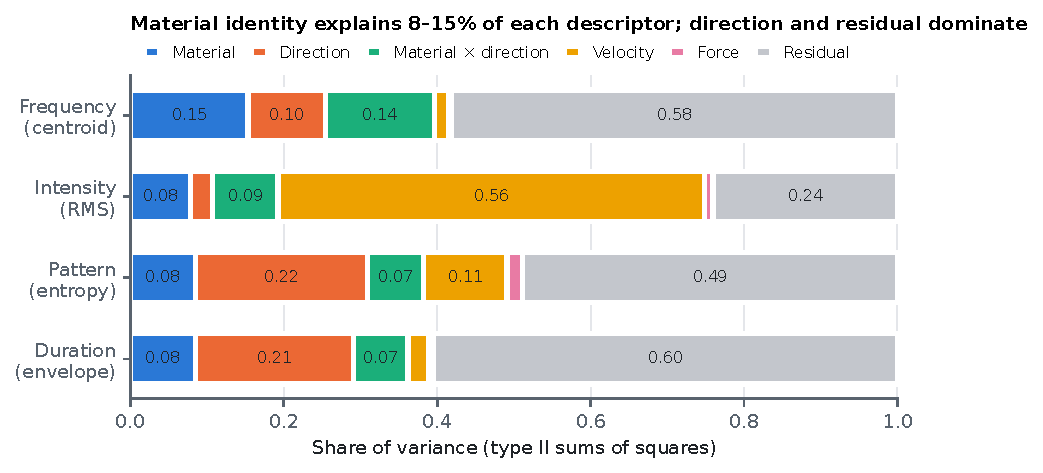
\includegraphics[width=\columnwidth]{fig1_variance_shares.pdf}
\caption{Share of each descriptor's variance explained by material, sliding
direction, their interaction, velocity, force and residual (type~II sums of
squares). Run \texttt{o1\_real\_analysis/20261104T155118\_372566Z}.}
\label{fig:var}
\end{figure}

\emph{Identity is in the signal, not the descriptor} (exploratory;
Fig.~\ref{fig:id}). With direction held out, logistic regression reaches 0.138 on
the four raw descriptors, 0.154 normalised, 0.218 on band powers and 0.248 on both
(chance 0.0625). The spectrogram CNN reaches $0.378$
% run o1_learned_baseline/20261106T214141_196418Z
(SD 0.003 over seeds, 0.080 over folds). With every direction seen in training it
reaches 0.542, so a held-out direction costs about a third of the accuracy. The
90$^\circ$ and 270$^\circ$ folds are hardest (0.27 and 0.24, against 0.39--0.45
for the other six); we did not test this pattern. Corduroy is identified best by
both model families (CNN recall 0.66), and cotton broadcloth and organdy worst
(0.14 and 0.23). The four-number descriptor therefore keeps well under half of
the fabric identity the signal carries. Even the CNN misidentifies most recordings
from an unseen direction.

\begin{figure}[t]
\centering
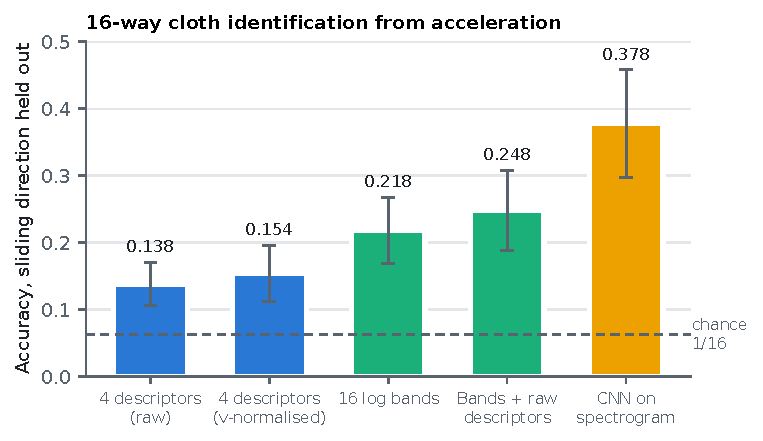
\includegraphics[width=\columnwidth]{fig4_identification.pdf}
\caption{16-way fabric identification with the sliding direction held out
(8 folds; error bars are SD over folds). Exploratory. Runs
\texttt{o1\_real\_analysis/20261104T155118\_372566Z} and
\texttt{o1\_learned\_baseline/20261106T214141\_196418Z}.}
\label{fig:id}
\end{figure}

\subsection{The centroid reflects the rig, not the surface}\label{sec:vel}
% run velocity_all_materials/20261105T202123_412283Z
Across all 118 materials, wood, stone and metal included, the centroid exponent
is near zero (Table~\ref{tab:vel}, Fig.~\ref{fig:vel} left). None of the 118 lies
within 0.25 of the $f=v/\lambda$ prediction, and 92\% lie within 0.25 of zero. The
non-cloth materials differ from 1 at $p=1.8\times10^{-18}$ (Wilcoxon). At
40~mm/s, every category's median centroid lies between 241 and 266~Hz. Categories
differ slightly (Kruskal--Wallis $p=1.2\times10^{-4}$), but cloth does not differ
from the rest ($p=0.13$). Because a spectral centroid that stays in one narrow
band at every speed, for every surface, cannot describe surface geometry, we read
it as the response of the probe and its mounting. As a result, the
velocity normalisation $\lambda=v/f$ makes descriptors \emph{more} velocity
dependent (coefficient of variation 0.40 against 0.06 for the raw centroid on
cloth).

Raw spectral-shift exponents tell the same story (median 0.16; none of 118 within
0.25 of 1). After whitening, the median over all materials is $-0.001$, but cloth
stands apart: median 0.22 against $-0.02$ for the rest (Mann--Whitney
$p=3.0\times10^{-4}$, cloth vs.\ zero $p=0.009$). We noticed this \emph{after}
plotting the data, so on its own it is post hoc.

\begin{table}[t]
\caption{Velocity exponent over 118 materials (directions 0$^\circ$/90$^\circ$,
first repeat). $f=v/\lambda$ predicts 1.}
\label{tab:vel}
\centering
\begin{tabular}{lcc}
\toprule
 & Centroid & Whitened shift \\
\midrule
Median, cloth (16) & $-0.039$ & $0.218$ \\
Median, other (102) & $-0.084$ & $-0.022$ \\
Within 0.25 of 1 & 0 / 118 & 0 / 118 \\
Cloth vs.\ rest (Mann--Whitney) & $p=0.13$ & $p=3.0\times10^{-4}$\,\textsuperscript{a} \\
\bottomrule
\multicolumn{3}{l}{\footnotesize \textsuperscript{a}Post hoc; confirmed on held-out data in Table~\ref{tab:confirm}.}
\end{tabular}
\end{table}

\begin{figure*}[t]
\centering
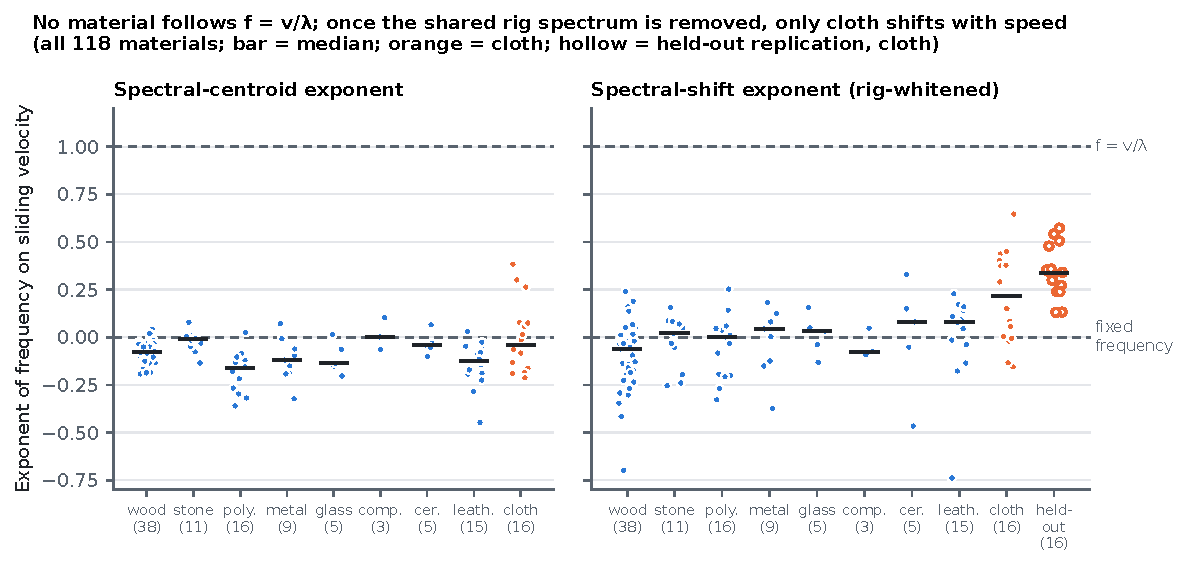
\includegraphics[width=0.9\textwidth]{fig3_velocity_exponents.pdf}
\caption{Velocity exponent per material by category. Left: spectral centroid.
Right: whitened spectral shift. Dashed lines mark 0 (no scaling) and 1
($f=v/\lambda$). Filled markers: discovery subset. Hollow: held-out cloth
recordings (pre-registered test). Runs
\texttt{velocity\_all\_materials/20261105T202123\_412283Z} and
\texttt{velocity\_confirm\_cloth/20261105T203252\_596852Z}.}
\label{fig:vel}
\end{figure*}

\subsection{Held-out replication: cloth spectra shift with velocity}\label{sec:confirm}
% run velocity_confirm_cloth/20261105T203252_596852Z
We tested two one-sided predictions on cloth recordings not used in the
discovery. They were fixed before the run but committed to the repository
afterwards, so we report this as a held-out replication, not a pre-registered
test: (1) the cloth whitened exponent exceeds 0;
(2) it exceeds that of the 102 other materials (from the discovery run). The
held-out data are cloth at the six other directions with both repeats, plus the
second repeat at 0$^\circ$ and 90$^\circ$: 2,240 recordings, 40 skipped, 444
(material, force, direction, repeat) cells. The whitening reference was taken from
the discovery subset only.

Both predictions hold (Table~\ref{tab:confirm}). All 16 fabrics shift upward, from
0.13 (mesh, chiffon) to 0.57 (corduroy), with cotton (0.54), lace (0.51) and velvet
(0.48) next. Measured against what all surfaces share, cloth spectra move up with
stroking speed by about a third of $v/\lambda$, and no other category's do.

\begin{table}[t]
\caption{Held-out replication (444 cells, 16 fabrics)}
\label{tab:confirm}
\centering
\begin{tabular}{lc}
\toprule
Median exponent [IQR] & 0.338 [0.258, 0.388] \\
Fabrics above 0 & 16 / 16 \\
(1) $>0$, Wilcoxon one-sided & $p=1.5\times10^{-5}$ (Holm $1.5\times10^{-5}$) \\
(2) $>$ others, Mann--Whitney & $p=5.4\times10^{-10}$ (Holm $1.1\times10^{-9}$) \\
\bottomrule
\end{tabular}
\end{table}

\subsection{Flatbed scans are not photographs}\label{sec:scan}
% runs o2_cluster_scans/20261104T161427_584869Z, o2_cluster_scan_scale/20261104T161606_361379Z
The MINC-trained classifier calls 75.6\% (189/250) of MINC's own fabric test
photographs ``fabric'', but only 3.25\% (52/1,600) of the cloth scan crops
(Fig.~\ref{fig:scan}). No fabric is classified as fabric by majority. Scans are
read as carpet (velvet, corduroy, wool), wallpaper (cotton, chiffon, lace, organdy)
or tile (mesh, linen). Field of view does not explain this: whole 100~mm scans give
1/16 and 50~mm quadrants 3/64. Texture attributes transfer better. Mapped onto the
pre-registered structural groups, DTD predictions on crops agree with the
by-eye labels 53\% of the time over all 16 fabrics, against 44\% for always
answering ``weave''. Corduroy is called pile in 99\% of crops.

\begin{figure}[t]
\centering
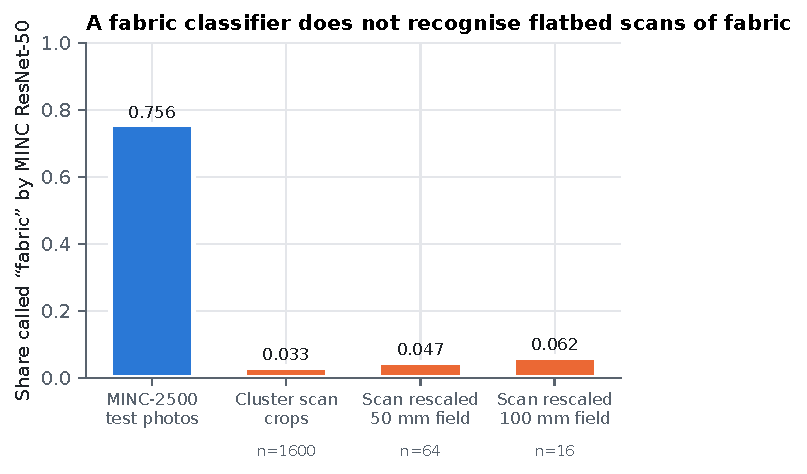
\includegraphics[width=\columnwidth]{fig2_scan_transfer.pdf}
\caption{``Fabric'' recall of a MINC-2500 ResNet-50 on MINC test photographs and on
Cluster's 300~dpi cloth scans at three fields of view. Runs
\texttt{o2\_cluster\_scans/20261104T161427\_584869Z} and
\texttt{o2\_cluster\_scan\_scale/20261104T161606\_361379Z}.}
\label{fig:scan}
\end{figure}

\subsection{Consequences for retrieval and rendering}
% runs o3_real/20261104T161615_092994Z, o4_fidelity_real/20261104T155413_654754Z
Two exploratory checks follow from the above. First, we retrieved the descriptor of
the most similar \emph{other} fabric, with the query fabric held out. Neither
class-pair lookup nor cosine similarity of image features beat predicting the mean
descriptor in any dimension. This is expected when descriptors barely separate
fabrics. Second, the browser vibration channel is on/off with a practical
10~ms tick, so it cannot switch faster than 25~Hz. Only 9 of 80 real cloth
envelopes have their modulation below that limit.

\subsection{Pre-registered follow-ups}\label{sec:round2}
Table~\ref{tab:round2} lists the six registered predictions; five held.

\emph{(A) Looks predict feel only through category.}
% run looks_feel/20261107T082554_607613Z
Over all 118 materials, visual and vibrotactile distances correlate weakly but
significantly ($r=+0.154$, Holm $p=0.0033$; 2,315 recordings). Permuting only
within category removes the effect (Holm $p=0.42$). Among the 16 fabrics the
correlation is $-0.095$ ($p=0.83$). Wood looks and feels unlike cloth, but which
fabric looks like which other fabric says nothing about which vibrates like which.
This matches the null retrieval result above. Generic image features are not
enough to choose a fabric's vibration.

\emph{(B) Contact audio carries more identity than acceleration.}
% run audio_vs_accel/20261107T110948_431117Z
On the same folds, full-band audio identifies the fabric in 72.0\% of recordings,
against 37.8\% for the acceleration baseline. Audio wins all 8 folds, by 0.22--0.45
(Wilcoxon $p=0.0039$). Restricted to 20--1000~Hz, audio still reaches 57.3\%. This
band-limited comparison was not part of the confirmatory test. Retraining on
acceleration with the same code gives 38.1\%, so the gap is not caused by the
training code. The microphone is a different sensor from the probe accelerometer.
The result therefore shows which recorded signal identifies a fabric best, not
which one feels right when rendered.

\emph{(C) A partial warp helps at an unseen speed.}
% run velocity_warp/20261107T111741_349222Z
With $k=0.338$, leave-one-velocity-out accuracy is 30.5\%, against 27.9\% unwarped
($k=0$) and 28.4\% for the full kinematic warp ($k=1$). The first prediction holds
(307 vs.\ 251 recordings, Holm $p=0.020$). The second does not: the advantage over
$k=1$ (331 vs.\ 292) is not significant ($p=0.064$). Every condition fails when
20~mm/s is held out (8.5--12.6\%), because that speed lies outside the training range.
Fold-to-fold SD (0.10--0.15) exceeds every difference between conditions.

\emph{(D) Benchmark.}
% runs benchmark118_linear/20261107T103411_132525Z, benchmark118_cnn/20261107T125519_960150Z
Table~\ref{tab:bench} gives baselines on 18,569 in-band recordings of all 118
materials. With direction held out, the CNN identifies the material in 20.2\% of
recordings (top-5 44.8\%; chance 0.85\%) and the category in 44.9\%, against a
majority baseline of 32.3\%. The four-number descriptor barely beats that baseline
at category level (34.7\%). Cloth is the most recognisable category (recall 0.71).
The three smallest categories, composite, glass and ceramic, are almost never
recognised (0.00--0.04).

\begin{table}[t]
\caption{Pre-registered follow-up predictions and outcomes}
\label{tab:round2}
\centering
\begin{tabular}{llc}
\toprule
Prediction & Test & Held \\
\midrule
(A) all 118 significant & Mantel, Holm $p=0.0033$ & yes \\
(A) within category n.s. & Mantel, Holm $p=0.42$ & yes \\
(A) cloth only n.s. & Mantel, $p=0.83$ & yes \\
(B) audio $>$ acceleration & Wilcoxon, $p=0.0039$ & yes \\
(C) $k=0.338>k=0$ & sign, Holm $p=0.020$ & yes \\
(C) $k=0.338>k=1$ & sign, Holm $p=0.064$ & no \\
\bottomrule
\multicolumn{3}{l}{\footnotesize Earlier registered tests: Tables~\ref{tab:gate} and \ref{tab:confirm}.}
\end{tabular}
\end{table}

\begin{table}[t]
\caption{118-material benchmark: accuracy (descriptive)}
\label{tab:bench}
\centering
\setlength{\tabcolsep}{4pt}
\begin{tabular}{llcccc}
\toprule
Task & Split & Descr. & Bands & Both & CNN \\
\midrule
Material (118) & direction & 0.031 & 0.078 & 0.083 & 0.202 \\
 & repeat & 0.035 & 0.107 & 0.111 & 0.338 \\
Category (9) & direction & 0.347 & 0.354 & 0.355 & 0.449 \\
 & repeat & 0.352 & 0.387 & 0.394 & 0.631 \\
\bottomrule
\multicolumn{6}{l}{\footnotesize Chance 0.0085 / 0.111; majority 0.009 / 0.323. CNN: mean of 3 seeds.}
\end{tabular}
\end{table}

% ---------------------------------------------------------------------------
\section{Discussion}

\emph{For rendering.} A per-fabric vibration signature built from a four-number
summary of this dataset would be close to the same signature for every fabric,
modulated mostly by speed. The CNN result shows that the recordings themselves
are more informative. A renderer that keeps more of the spectrum, or that conditions
on direction, has room to do better. Direction is a large, structured source of
variance, plausibly reflecting warp and weft, but we have not tested this.
The audio result (B) suggests a practical route. A renderer driven by the contact
audio, band-limited to what the actuator can play, starts from a signal that
separates fabrics better than acceleration. Whether it also \emph{feels} more
distinct is a perceptual question that we have not tested.

\emph{For image-to-vibration retrieval.} Analysis A sets a ceiling on approaches
that use generic image features. Within cloth, visual similarity is unrelated to
vibrotactile similarity, so any retrieval gain must come from features trained on
the tactile side, not from ImageNet similarity. For speed, the confirmed partial
exponent is useful in practice: warping by it helps at an unseen speed (C), but
not beyond the measured range.

\emph{For the dataset.} The 240--270~Hz centroid common to all 118 surfaces, and
its insensitivity to speed, should be accounted for by anyone who uses the
acceleration channel for texture. Whitening against the cross-material median is a
simple correction, and it reveals a velocity effect that the raw centroid hides.

\emph{What the confirmed effect is not.} A partial shift of the whole log spectrum
(slope about 0.34 rather than 1) does not by itself identify a mechanism. It is
consistent with a texture component that scales as $v/\lambda$ mixed with a
fixed one. It is equally consistent with a speed-dependent change of spectral tilt,
for instance through damping by a compliant fabric. Telling these apart needs
surface profiles, which the dataset does not provide. The ordering of fabrics
(coarse structures high, sheer fabrics low) is descriptive and was not predicted.

\emph{Limitations.} One rig and one dataset; the rig dependence we report may not
hold elsewhere. The whitening reference includes the 16 fabrics themselves (16 of
118 materials); this works against finding a cloth-specific effect, not for it.
Group labels were assigned by eye. The 16-fabric identification analyses are
exploratory; the round-2 benchmark is descriptive. In (A), the visual side uses
the dataset's own crops, which are scans, not product photographs. We have measured the scan$\to$photo gap only in the direction
photograph-trained model $\to$ scans. The reverse direction, which matters for
shopping, needs labelled product photographs, which we have not collected. No
perceptual data are reported. Whether people can feel the differences that survive
is the subject of a planned user study.

% ---------------------------------------------------------------------------
\section{Conclusion}

On the 16 cloth materials of the Cluster dataset, compact vibrotactile descriptors
do not separate fabrics, although the signal carries identity that a spectrogram
CNN partly recovers. The probe's spectral centroid is a property of the rig, not
of the surface. Measured against the response shared by all surfaces, cloth
spectra shift with speed in a way that replicates on held-out recordings.
Image models trained on photographs do not recognise the dataset's scans as
fabric, and their visual similarity does not predict vibrotactile similarity
between fabrics. Contact audio identifies fabrics better than acceleration. A
speed warp using the confirmed exponent helps recognition at unseen speeds. Each of
these findings constrains how the dataset can be used for
vibrotactile shopping applications.

\section*{Data and Code Availability}
The dataset is public~\cite{cluster2026}. Code, saved runs (with configuration,
code version and metrics), figures and the pre-registration are available at
\url{https://github.com/Jashwanth1255/haptic-project}. % TODO(team): archive a release (e.g. Zenodo DOI) before submission
Every number in this paper names the run it comes from.

\bibliographystyle{IEEEtran}
\bibliography{references}

\end{document}
